\hypertarget{sorting-algorithms}{%
\section{Sorting Algorithms}\label{sorting-algorithms}}

\begin{itemize}
\tightlist
\item
  sorting can be \textbf{comparison-based or non-comparison-based}
\item
  the fundamental operation of comparison-based sorting is
  compare-exchange
\item
  the lower bound on any comparison-based sequential sorting of n
  numbers is $\mathcal{O}(n * log (n))$
\item
  we focus here on comparison-based sorting algorithms
\end{itemize}

\hypertarget{compare-exchangesplit}{%
\subsection{Compare-Exchange/Split}\label{compare-exchangesplit}}

\hypertarget{compare-exchange}{%
\subsubsection{Compare Exchange}\label{compare-exchange}}

\begin{figure}[H]
\centering
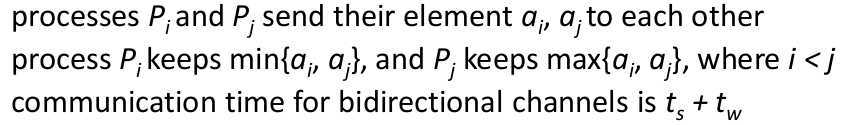
\includegraphics[width=0.6\textwidth]{figures/compareExchange.png}
\caption{Compare Exchange process}
\end{figure}

\hypertarget{compare-split}{%
\subsubsection{Compare Split}\label{compare-split}}

\begin{figure}[H]
\centering
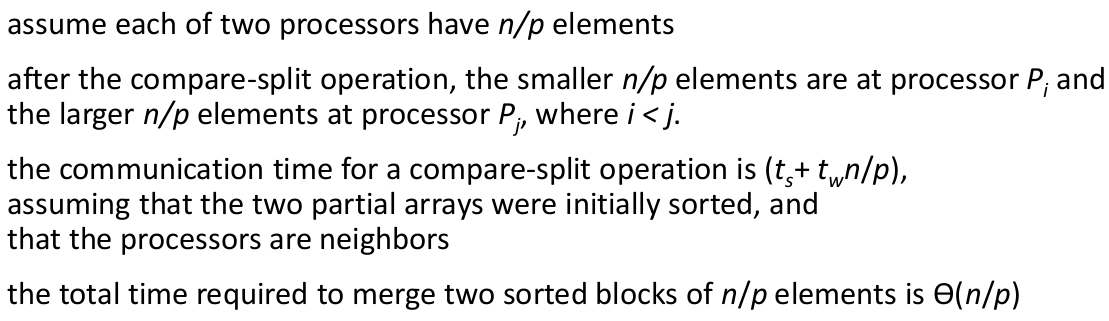
\includegraphics[width=0.8\textwidth]{figures/comparesplit.png}
\caption{Compare Split process}
\end{figure}

\begin{figure}[H]
\centering
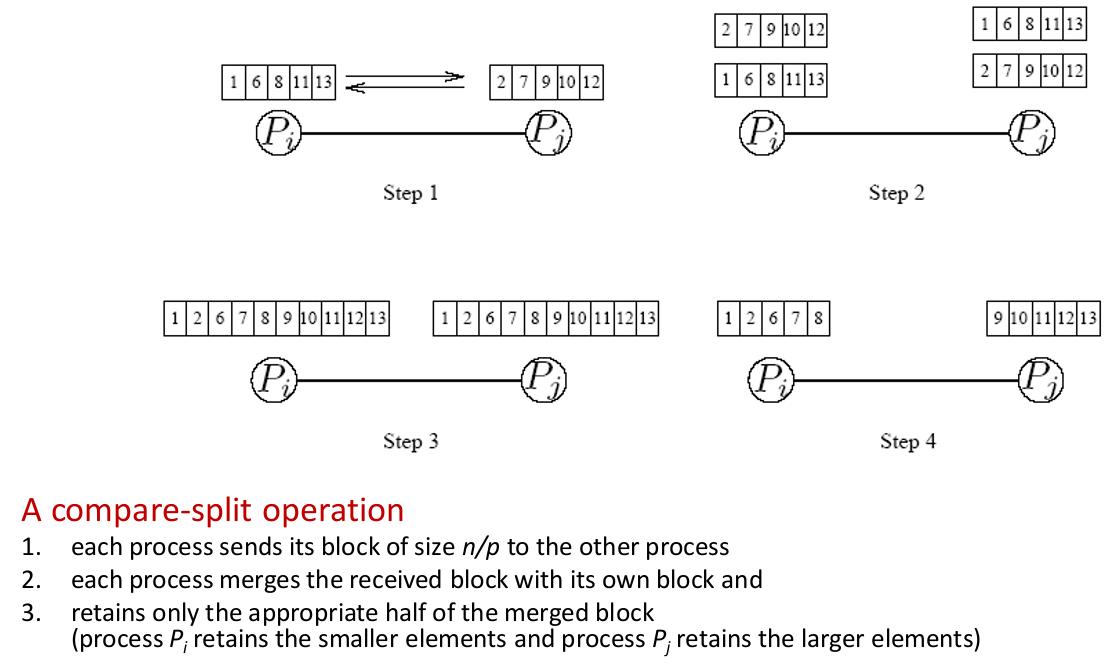
\includegraphics[width=0.8\textwidth]{figures/comparesplitExample.png}
\caption{Compare Split example}
\end{figure}

\hypertarget{odd-even-transposition-sort}{%
\subsection{Odd-Even Transposition
Sort}\label{odd-even-transposition-sort}}

\begin{figure}[H]
\centering
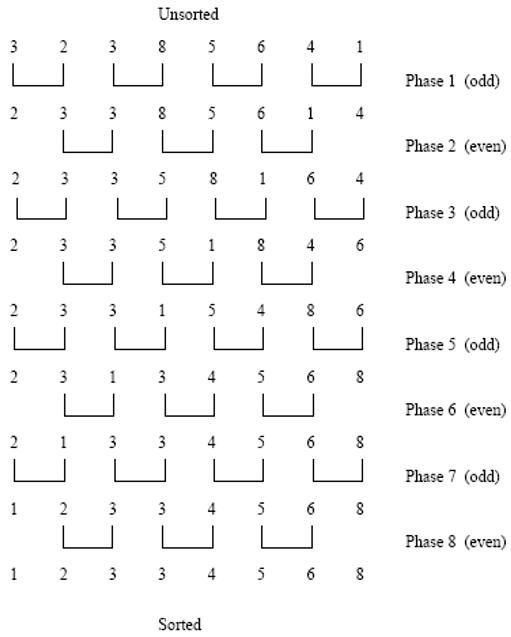
\includegraphics[width=0.4\textwidth]{figures/transpositionsort.png}
\caption{Odd-Even Transposition Sort}
\end{figure}

\hypertarget{parallel-shellsort}{%
\subsection{Parallel Shellsort}\label{parallel-shellsort}}

\begin{itemize}
\tightlist
\item
  let n be the number of elements to be sorted and p be the number of
  processes
\item
  during the first phase, processes that are far away from each other in
  the array compare split their elements
\item
  during the second phase, the algorithm switches to an odd-even
  transposition sort with $2l \leq p$ iterations
\end{itemize}

In phase 1:

\begin{itemize}
\tightlist
\item
  initially, each process sorts its block of $n/p$ elements internally
\item
  each process is now paired with its corresponding process in the
  reverse order of the array: that is, process $P_i$ is paired with
  process $P_{p-i-1}$, where $i < p/2$
\item
  all pairs perform a compare-split operation
\item
  the processes are split into two groups of size $p/2$ each and the phase
  1 is repeated in each group until a group contains one process only
\end{itemize}

\begin{figure}[H]
\centering
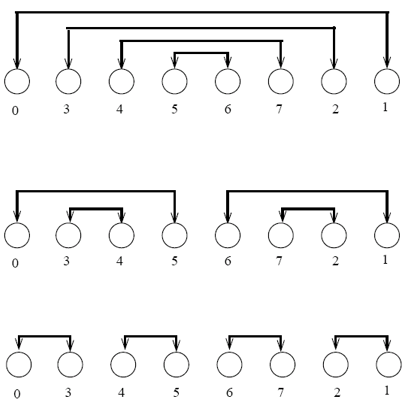
\includegraphics[width=0.35\textwidth]{figures/parallelshellsort.png}
\caption{Parallel Shellsort}
\end{figure}

\begin{itemize}
\tightlist
\item
  In the first phase, each process performs $d = log(p)$ compare-split
  operations
\item
  with $\mathcal{O}(p)$ bisection width, each communication can be performed in time   $\Theta(n/p)$ for a total time of $\Theta ( \frac{n * log (p)}{p})$
\item
  in the second phase, l odd and l even iterations are performed, each
  requiring time $\Theta(n/p)$
\end{itemize}

\begin{figure}[H]
\centering
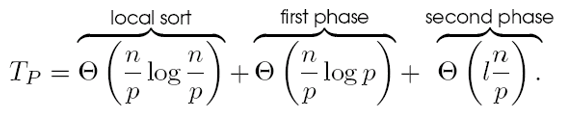
\includegraphics[width=0.4\textwidth]{figures/runtimeShellsort.png}
\caption{Parallel runtime of Shellsort}
\end{figure}

\clearpage
\hypertarget{sorting-networks}{%
\subsection{Sorting Networks}\label{sorting-networks}}

\begin{itemize}
\tightlist
\item
  a sorting network is a network of comparators designed specifically
  for sorting
\item
  a comparator is a device with

  \begin{itemize}
  \tightlist
  \item
    2 inputs: $x$ and $y$
  \item
    2 outputs: $x'$ and $y'$
  \end{itemize}
\item
  an increasing comparator $\oplus : x' = min\{x,y\} and y' = max\{x,y\}$
\item
  a decreasing comparator $\ominus : x' = max\{x,y\} and y' = min\{x,y\}$
\end{itemize}

\begin{figure}[H]
\centering
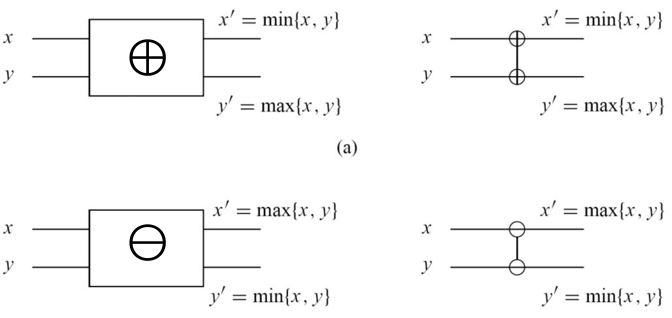
\includegraphics[width=0.7\textwidth]{figures/sortingNetwork.png}
\caption{Sorting Networks}
\end{figure}

\begin{figure}[H]
\centering
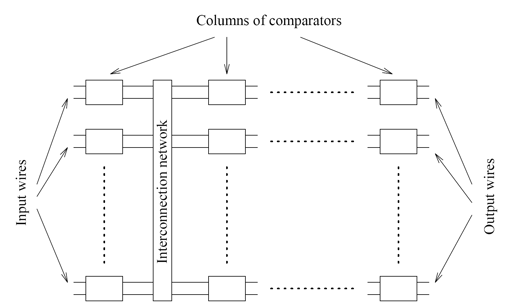
\includegraphics[width=0.7\textwidth]{figures/sortingNetwork2.png}
\caption{Sorting Network Example}
\end{figure}

\clearpage
\hypertarget{bitonic-sort}{%
\subsection{Bitonic Sort}\label{bitonic-sort}}

A bitonic sequence has two tones (sequences), one increasing and one
decreasing or vice versa. Any cyclic rotation fo a bitonic sequence is
also bitonic (repeated sequence). E.g. \{1,2,4,7,6,0\} is bitonic or
\{8,9,2,1,0,4\} is bitonic (because it's repeated).

For the bitonic sort, we

\begin{enumerate}
\def\labelenumi{\arabic{enumi}.}
\tightlist
\item
  build a single bitonic sequence from the given unsorted sequence
\item
  rearrange the bitonic sequence into a sorted sequence
\end{enumerate}

Parallel Runtime (p = n): a bitonic sorting network sorts n elements in
$\Theta(log^2 (n))$ time.

\hypertarget{bitonic-merge}{%
\subsubsection{Bitonic Merge}\label{bitonic-merge}}

\begin{figure}[H]
\centering
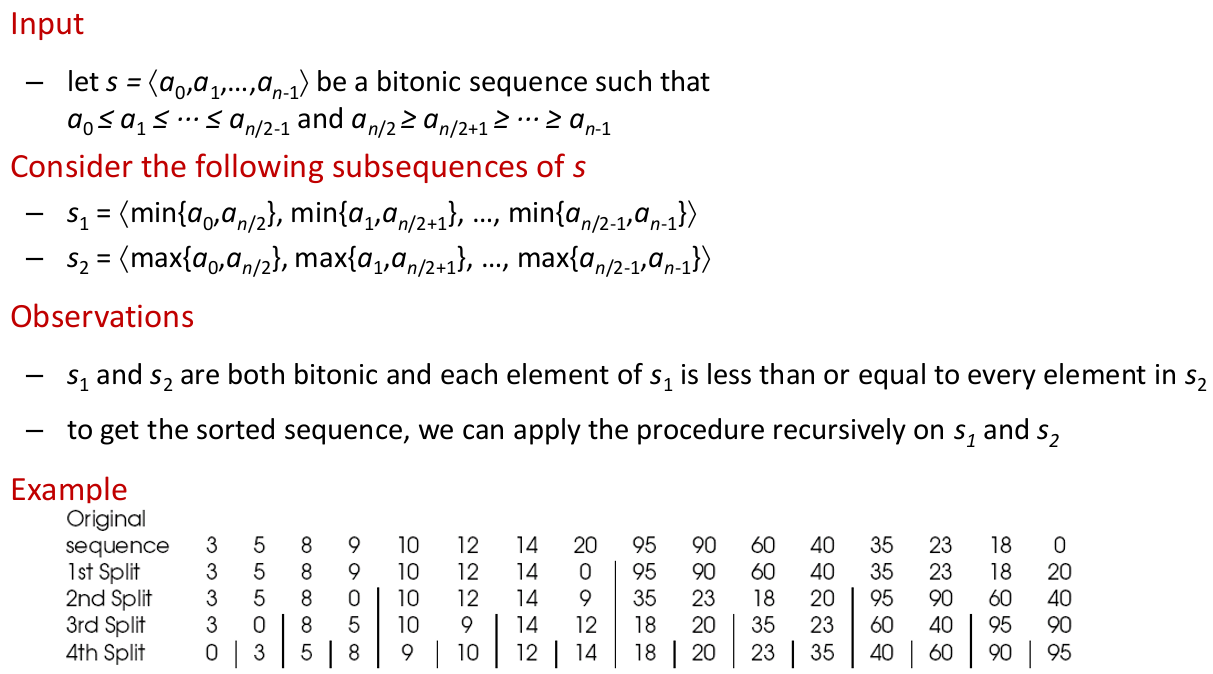
\includegraphics[width=0.9\textwidth]{figures/bitonicSequenceTheory.png}
\caption{Theory Bitonic Merge}
\end{figure}

In other words: At the beginning, there is one big bitonic sequence. In
splitting this bitonic sequence into two, you have two new sequences
(lower and upper sequence). If you repeate this splitting, you will have
a sorted sequence at the end.

\begin{figure}[H]
\centering
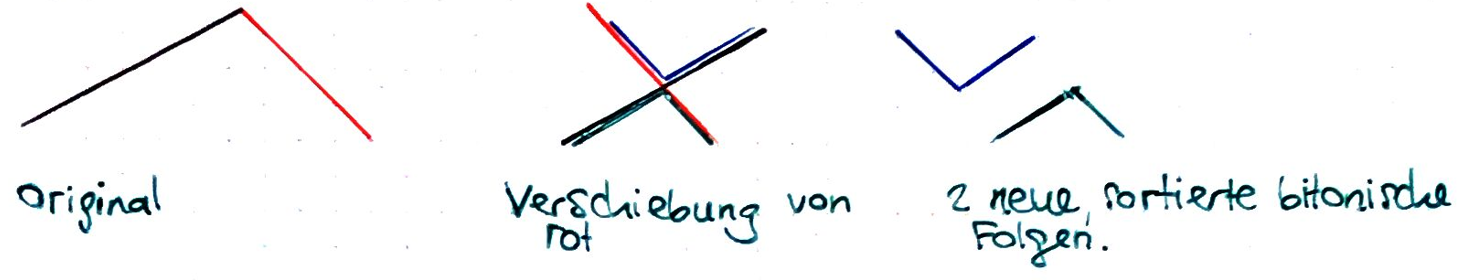
\includegraphics[width=0.9\textwidth]{figures/bitonic-merge.png}
\caption{Bitonic Merge}
\end{figure}

\clearpage
\hypertarget{building-a-bitonic-sequence}{%
\subsubsection{Building a Bitonic
Sequence}\label{building-a-bitonic-sequence}}

\begin{figure}[H]
\centering
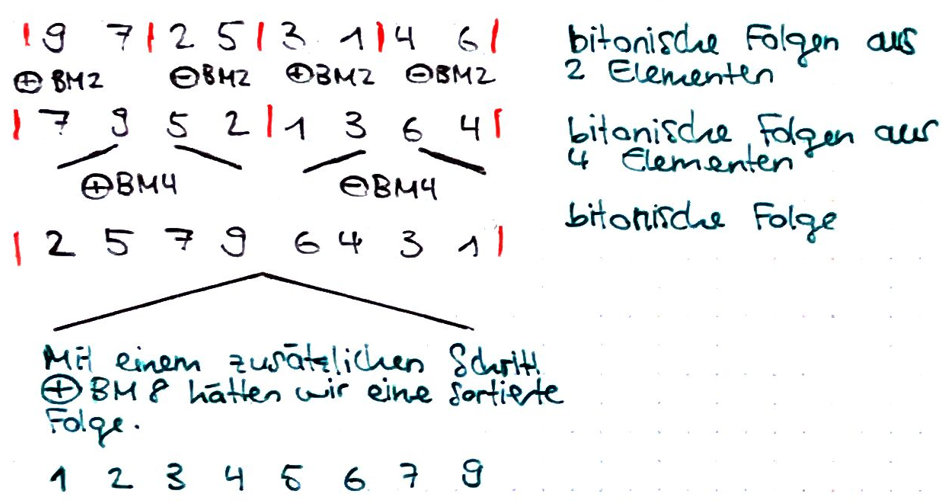
\includegraphics[width=0.7\textwidth]{figures/create-bitonic-sequence.png}
\caption{Creation of a bitonic sequence}
\end{figure}

\hypertarget{bitonic-sort-block-of-elements-per-process}{%
\subsubsection{Bitonic Sort: Block of Elements Per
Process}\label{bitonic-sort-block-of-elements-per-process}}

You are also able to implement bitonic sort if there are less processes
than elements.

\begin{itemize}
\tightlist
\item
  the first step is a local sort of the local block
\item
  each subsequent compare-exchange operation is replaced by a
  compare-split operation
\item
  the bitonic network consists of $(1 + log (p))*\frac{log (p)}{2} = \mathcal{O}(log^2 (p))$
  steps
\end{itemize}

\hypertarget{parallel-quicksort}{%
\subsection{Parallel Quicksort}\label{parallel-quicksort}}

The following figure describes the serial sequence of the quick sort.

\begin{figure}[H]
\centering
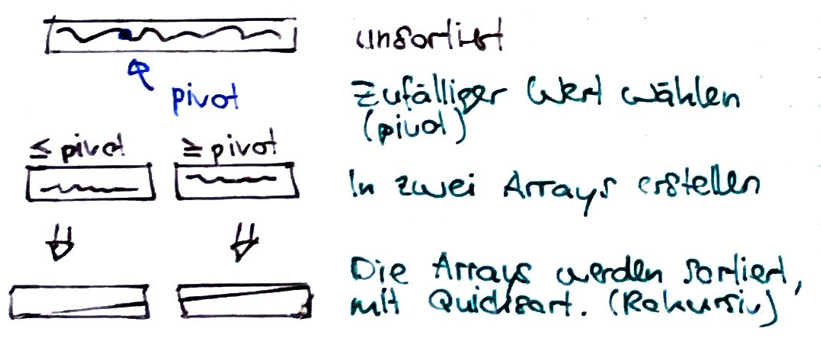
\includegraphics[width=0.7\textwidth]{figures/quicksort-serial.png}
\caption{Quicksort in Serial}
\end{figure}

\clearpage
\hypertarget{recursive-decomposition}{%
\subsubsection{Recursive Decomposition}\label{recursive-decomposition}}

\begin{itemize}
\tightlist
\item
  the array is partitioned serially and each of the sub-problems is
  handled by a different process
\item
  the time for this algorithm is lower-bounded by $\Omega(n)$, because of the serial partitioning
\end{itemize}

\begin{figure}[H]
\centering
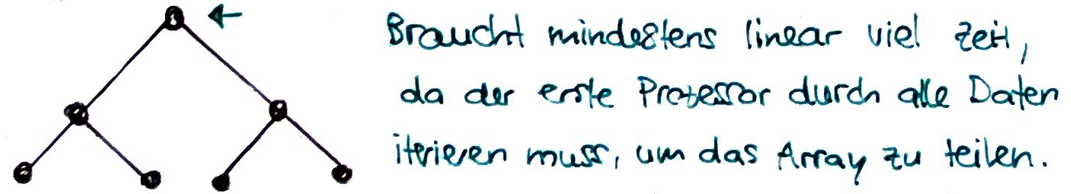
\includegraphics[width=0.7\textwidth]{figures/quicksort-parallel.png}
\caption{Quicksort in parallel}
\end{figure}

\hypertarget{pram}{%
\subsubsection{PRAM}\label{pram}}

PRAM makes use of CRCW (concurrent read, concurrent write).

\begin{itemize}
\tightlist
\item
  process $P_i$ is assigned element $A[i]$
\item
  build binary tree
\item
  traverse tree and count elements in left and right sub-trees and
  compute correct element positions
\item
  each process writes its element to the correct position in A
\end{itemize}

\begin{figure}[H]
\centering
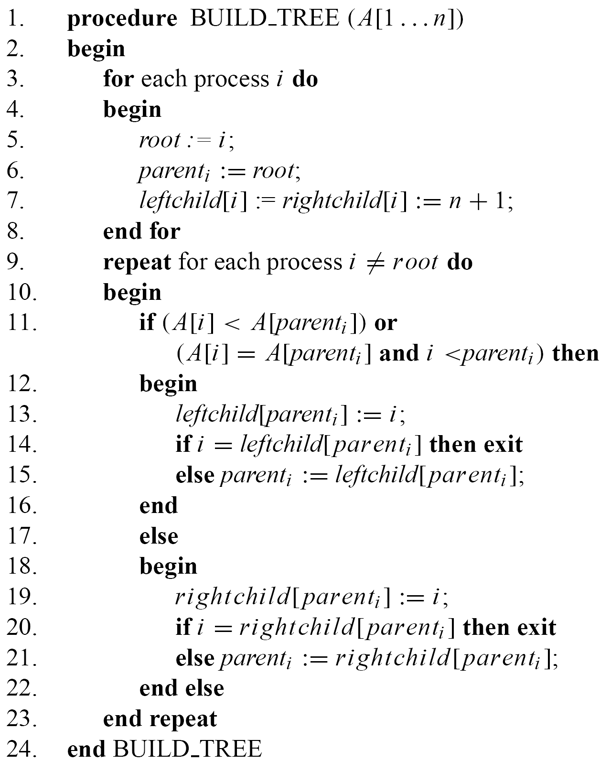
\includegraphics[width=0.4\textwidth]{figures/quicksortPRAM.png}
\caption{Quicksort PRAM pseudo-code}
\end{figure}

\begin{itemize}
\tightlist
\item
  The arbitrary choice of root (by concurrent write of all processes) is
  the new pivot
\item
  The root doesn't work anymore.
\item
  All other processes save their value into the proper array of the
  existing two halfs
\end{itemize}

\begin{figure}[H]
\centering
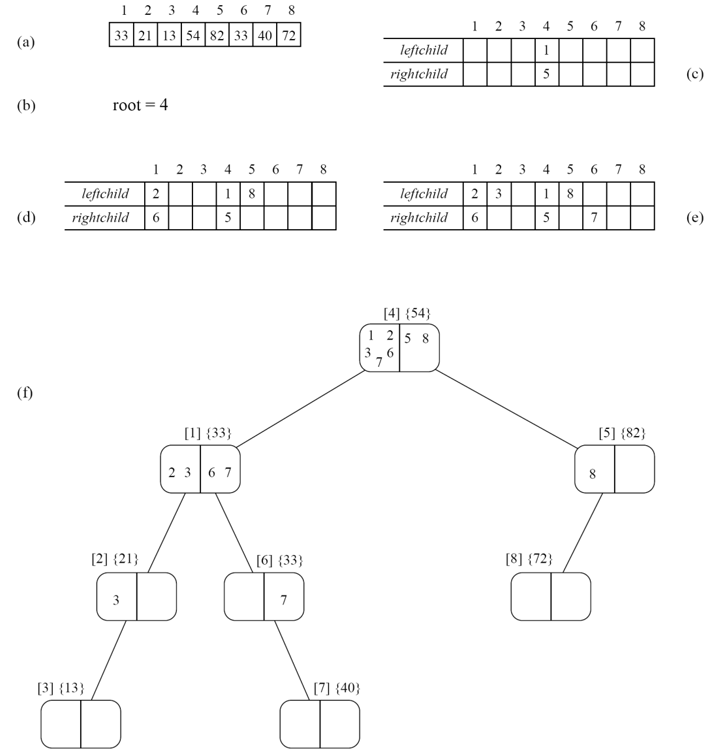
\includegraphics[width=0.7\textwidth]{figures/binarytreeQuicksortExample.png}
\caption{Quicksort Example Binary tree}
\end{figure}

\begin{itemize}
\tightlist
\item
  As soon as the binary tree is created, the values need to be written
  to the goal array
\item
  Each node needs to know his final position in the goal array
\item
  The position can be calculated from the left childs of the current
  node
\item
  The number of childs can be calculated recursively by asking his child
  how many child it has (which asks his childs again\ldots{})
\end{itemize}

\clearpage
\hypertarget{shared-address-space-sas-parallelizing-quicksort}{%
\subsubsection{Shared Address Space (SAS): Parallelizing
Quicksort}\label{shared-address-space-sas-parallelizing-quicksort}}

Consider an array of size n equally divided across p processes.

\begin{itemize}
\tightlist
\item
  Pivot Selection

  \begin{itemize}
  \tightlist
  \item
    a pivot is selected by one of the processes and made known to all
    processes
  \item
    can be made local from one process
  \end{itemize}
\item
  Local Rearrangement

  \begin{itemize}
  \tightlist
  \item
    each process partitions its array block into two, say S\_i and L\_i
    , based on the selected and communicated pivot
  \end{itemize}
\item
  Global Rearrangement

  \begin{itemize}
  \tightlist
  \item
    all of the S\_i arrays are merged to S and all of the L\_i arrays
    are merged to L separately
  \end{itemize}
\item
  Processor Partitioning

  \begin{itemize}
  \tightlist
  \item
    the set of processes is partitioned into two (in proportion of the
    size of arrays S and L)
  \end{itemize}
\item
  the algorithm is recursively repeated for each process group and
  sub-array, until a sub-array is assigned to a single process, in which
  case it proceeds to sort it locally
\end{itemize}

\begin{figure}[H]
\centering
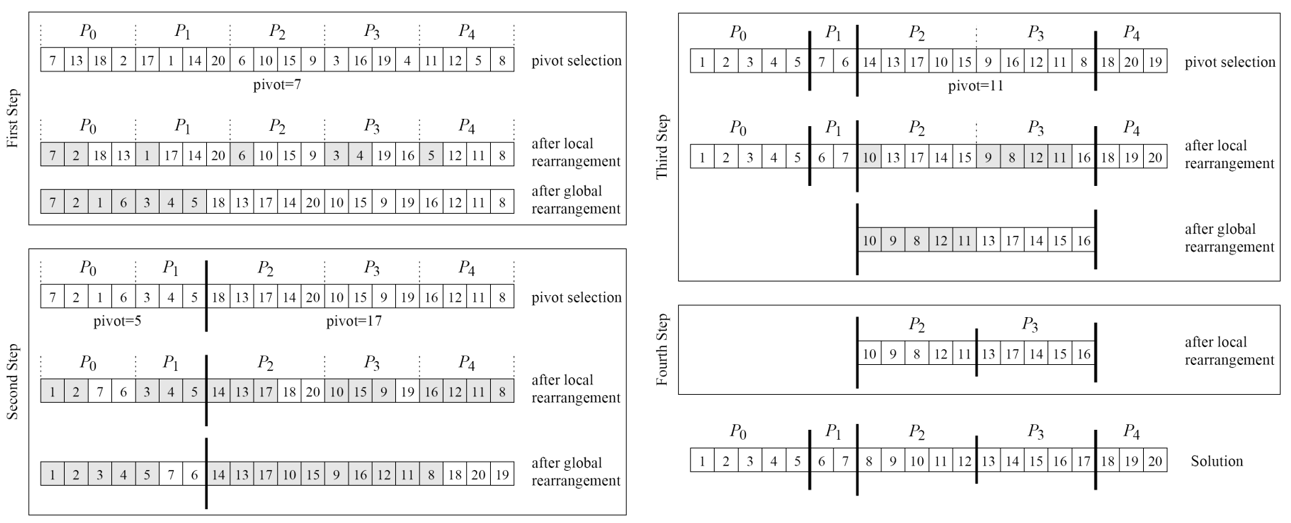
\includegraphics[width=1\textwidth]{figures/quicksortSASExample.png}
\caption{SAS Quicksort Example}
\end{figure}

\begin{figure}[H]
\centering
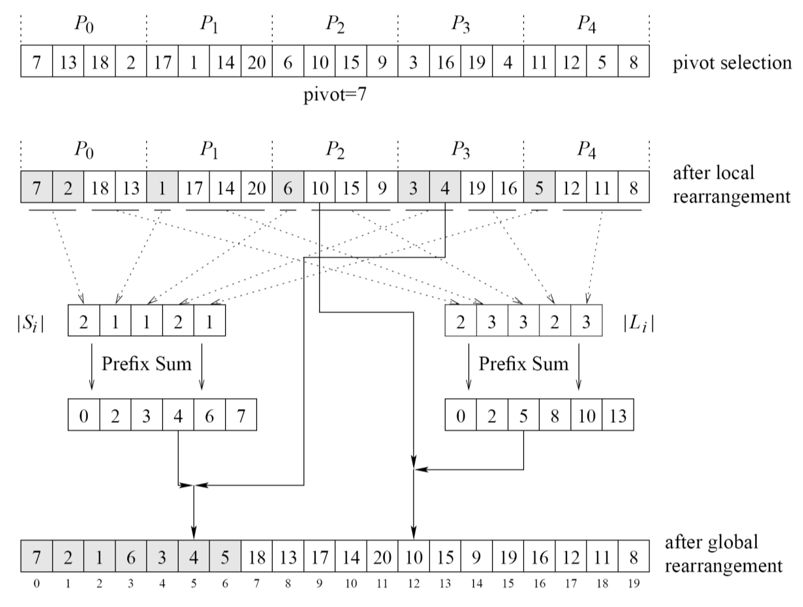
\includegraphics[width=0.6\textwidth]{figures/sasQuicksortGlobalRearrangement.png}
\caption{SAS Quicksort Global Rearrangement}
\end{figure}

\hypertarget{bucket-sort}{%
\subsection{Bucket Sort}\label{bucket-sort}}

The sequential bucket sort divides the values which need to be sorted
into different buckets. After that, one can sort the buckts itself.

\begin{figure}[H]
\centering
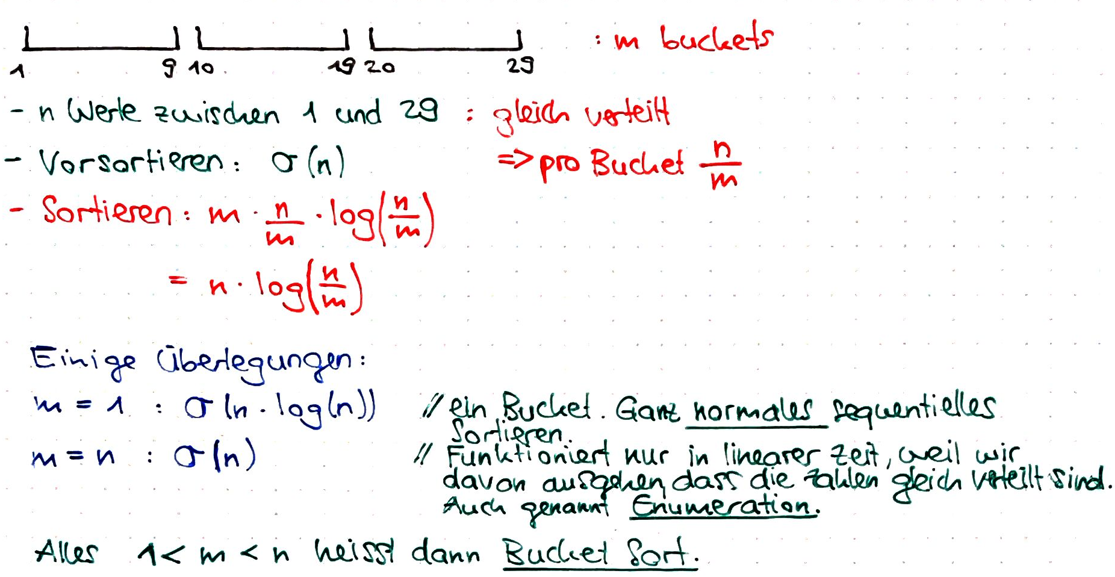
\includegraphics[width=0.9\textwidth]{figures/bucket-sort.png}
\caption{Bucketsort}
\end{figure}

\clearpage
\hypertarget{parallel-bucket-sort}{%
\subsubsection{Parallel Bucket Sort}\label{parallel-bucket-sort}}

The pre-sorting into different buckets can also be done in parallel.

\begin{itemize}
\tightlist
\item
  Input

  \begin{itemize}
  \tightlist
  \item
    each process is assigned a block of $n/p$ elements
  \item
    the number of buckets $m = p$
  \item
    each process knows the range $[a, b]$
  \end{itemize}
\item
  Algorithm

  \begin{itemize}
  \tightlist
  \item
    each process partitions its block of $n/p$ elements into p sub-blocks, one for each of the $p$ buckets: $\Theta(n/p)$
  \item
    each process sends $p- 1$ sub-blocks to the appropriate processes
    using a single all-to-all personalized communication: $\Theta(p * n/p^2) = \Theta(n/p)$
  \item
    each process sorts all the elements it receives by using an optimal
    sequential sorting algorithm: $\Theta((n/p) * log (n/p))$
  \end{itemize}
\item
  Parallel Runtime

  \begin{itemize}
  \tightlist
  \item
    $T_P = \Theta(n/p) + \Theta(n/p) + \Theta((n/p) *log (n/p)) = \Theta((n/p) * log (n/p))$
  \end{itemize}
\end{itemize}


\clearpage
\hypertarget{sample-sort}{%
\subsection{Sample Sort}\label{sample-sort}}

\begin{tcolorbox}[colback=red!5!white,colframe=red!75!black]
Random Sampling: If I don't know the distribution of my data, I can take a random sequence of this data ond check the distribution of this sequence, with the assumption that it is the same as the rest of the data. 
\end{tcolorbox}

\begin{itemize}
\tightlist
\item
  Similar to Bucket Sort

  \begin{itemize}
  \tightlist
  \item
    without the unrealistic assumption of uniformly distributed elements
  \item
    a sample is selected from the n elements, and the range of the
    buckets is determined by choosing m - 1 elements (splitters) from
    the sample
  \end{itemize}
\item
  Splitter Selection Method

  \begin{itemize}
  \tightlist
  \item
    the n elements are divided into m blocks of size n/m each
  \item
    each block is sorted by using an optimal sequential sorting
    algorithm
  \item
    from each sorted block m - 1 evenly spaced elements are chosen
  \item
    the m(m - 1) elements selected from all the blocks represent the
    sample used to determine the buckets
  \item
    from the sorted sample choose m - 1 evenly spaced splitters
  \item
    this scheme guarantees that the number of elements ending up in each
    bucket is less than 2n/m if the elements don't contain duplicates
  \end{itemize}
\end{itemize}

\begin{figure}[H]
\centering
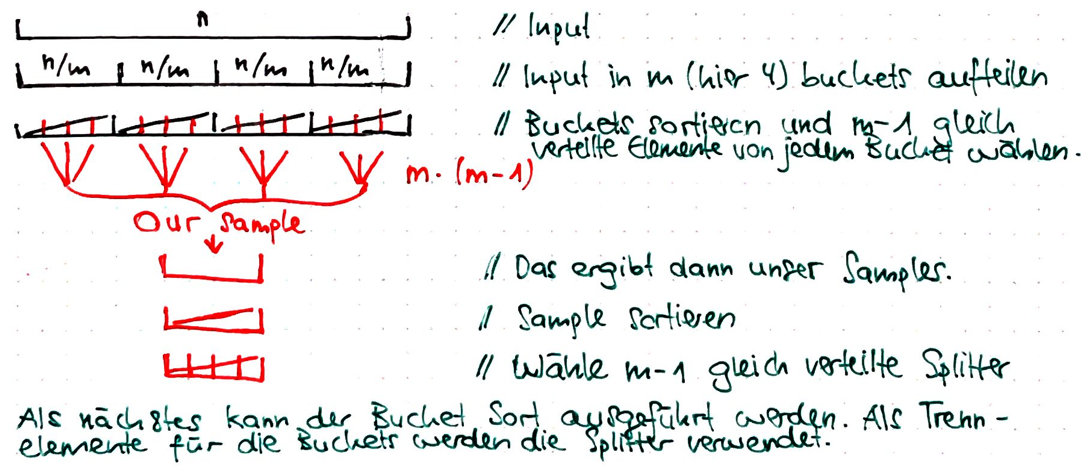
\includegraphics[width=0.9\textwidth]{figures/samplesort.png}
\caption{Samplesort}
\end{figure}

\clearpage
\hypertarget{parallel-sample-sort}{%
\subsubsection{Parallel Sample Sort}\label{parallel-sample-sort}}

\begin{itemize}
\tightlist
\item
  Parallelized Splitter Selection Scheme

  \begin{itemize}
  \tightlist
  \item
    choose $m = p$
  \item
    each processor generates the $p - 1$ local splitters in parallel
  \item
    all processors share their splitters using a single all-to-all
    broadcast operation
  \item
    each processor sorts (merges) the same $p*(p- 1)$ sorted sample
    elements it receives and selects the same $p - 1$ uniformly spaces
    splitters from them
  \end{itemize}
\item
  Parallel Algorithm

  \begin{itemize}
  \tightlist
  \item
    each process partitions its block of $n/p$ elements into p sub-blocks
    according to the $p - 1$ splitters, one for each of the p buckets
  \item
    each process sends p sub-blocks to the appropriate processes (a
    single all-to-all personalized communication is useful only if all
    sub-blocks are of almost equal size)
  \item
    each process merges all the received p sub-blocks
  \end{itemize}
\end{itemize}

\hypertarget{analysis-of-sample-sort}{%
\subsubsection{Analysis of Sample Sort}\label{analysis-of-sample-sort}}

\begin{figure}[H]
\centering
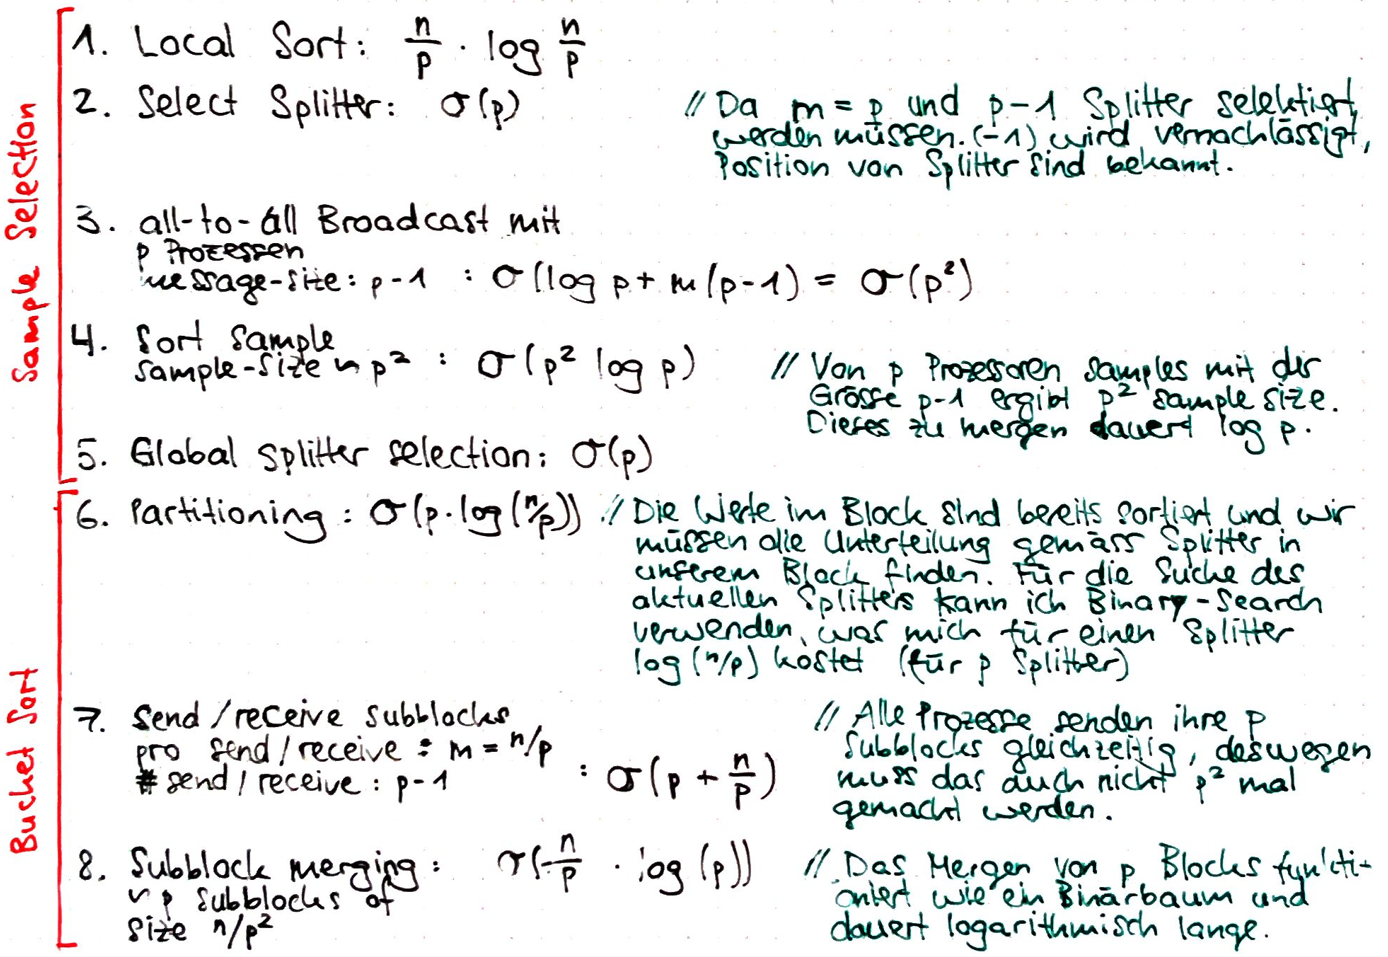
\includegraphics[width=0.85\textwidth]{figures/analysis-samplesort.png}
\caption{Analysis of the sample-sort}
\end{figure}

\textbf{Total} $= \mathcal{O}(\frac{n}{p}*log(\frac{n}{p}))+\mathcal{O}(p^2 * log(p)) + \mathcal{O}(p * log(\frac{n}{p})) + \mathcal{O}(\frac{n}{p} * log(p))$ \\
$= \mathcal{O}(\frac{n}{p}*log(n)) + \mathcal{O}(p^2*log(p)) + \mathcal{O}(p*log(\frac{n}{p}))$\\ \\ 
Da gilt: $\mathcal{O}(\frac{n}{p}*log (\frac{n}{p})) = \mathcal{O}(\frac{n}{p}*log(n) - \frac{n}{p}*log(p))$